\documentclass[twoside]{book}

% Packages required by doxygen
\usepackage{calc}
\usepackage{doxygen}
\usepackage{graphicx}
\usepackage[utf8]{inputenc}
\usepackage{makeidx}
\usepackage{multicol}
\usepackage{multirow}
\usepackage{textcomp}
\usepackage[table]{xcolor}

% Font selection
\usepackage[T1]{fontenc}
\usepackage{mathptmx}
\usepackage[scaled=.90]{helvet}
\usepackage{courier}
\usepackage{amssymb}
\usepackage{sectsty}
\renewcommand{\familydefault}{\sfdefault}
\allsectionsfont{%
  \fontseries{bc}\selectfont%
  \color{darkgray}%
}
\renewcommand{\DoxyLabelFont}{%
  \fontseries{bc}\selectfont%
  \color{darkgray}%
}

% Page & text layout
\usepackage{geometry}
\geometry{%
  a4paper,%
  top=2.5cm,%
  bottom=2.5cm,%
  left=2.5cm,%
  right=2.5cm%
}
\tolerance=750
\hfuzz=15pt
\hbadness=750
\setlength{\emergencystretch}{15pt}
\setlength{\parindent}{0cm}
\setlength{\parskip}{0.2cm}
\makeatletter
\renewcommand{\paragraph}{%
  \@startsection{paragraph}{4}{0ex}{-1.0ex}{1.0ex}{%
    \normalfont\normalsize\bfseries\SS@parafont%
  }%
}
\renewcommand{\subparagraph}{%
  \@startsection{subparagraph}{5}{0ex}{-1.0ex}{1.0ex}{%
    \normalfont\normalsize\bfseries\SS@subparafont%
  }%
}
\makeatother

% Headers & footers
\usepackage{fancyhdr}
\pagestyle{fancyplain}
\fancyhead[LE]{\fancyplain{}{\bfseries\thepage}}
\fancyhead[CE]{\fancyplain{}{}}
\fancyhead[RE]{\fancyplain{}{\bfseries\leftmark}}
\fancyhead[LO]{\fancyplain{}{\bfseries\rightmark}}
\fancyhead[CO]{\fancyplain{}{}}
\fancyhead[RO]{\fancyplain{}{\bfseries\thepage}}
\fancyfoot[LE]{\fancyplain{}{}}
\fancyfoot[CE]{\fancyplain{}{}}
\fancyfoot[RE]{\fancyplain{}{\bfseries\scriptsize Generated on Wed Dec 16 2015 00\-:46\-:03 for R\-A\-P\-P Platform Tests -\/ Speech Detection Google by Doxygen }}
\fancyfoot[LO]{\fancyplain{}{\bfseries\scriptsize Generated on Wed Dec 16 2015 00\-:46\-:03 for R\-A\-P\-P Platform Tests -\/ Speech Detection Google by Doxygen }}
\fancyfoot[CO]{\fancyplain{}{}}
\fancyfoot[RO]{\fancyplain{}{}}
\renewcommand{\footrulewidth}{0.4pt}
\renewcommand{\chaptermark}[1]{%
  \markboth{#1}{}%
}
\renewcommand{\sectionmark}[1]{%
  \markright{\thesection\ #1}%
}

% Indices & bibliography
\usepackage{natbib}
\usepackage[titles]{tocloft}
\setcounter{tocdepth}{3}
\setcounter{secnumdepth}{5}
\makeindex

% Hyperlinks (required, but should be loaded last)
\usepackage{ifpdf}
\ifpdf
  \usepackage[pdftex,pagebackref=true]{hyperref}
\else
  \usepackage[ps2pdf,pagebackref=true]{hyperref}
\fi
\hypersetup{%
  colorlinks=true,%
  linkcolor=blue,%
  citecolor=blue,%
  unicode%
}

% Custom commands
\newcommand{\clearemptydoublepage}{%
  \newpage{\pagestyle{empty}\cleardoublepage}%
}


%===== C O N T E N T S =====

\begin{document}

% Titlepage & ToC
\hypersetup{pageanchor=false}
\pagenumbering{roman}
\begin{titlepage}
\vspace*{7cm}
\begin{center}%
{\Large R\-A\-P\-P Platform Tests -\/ Speech Detection Google \\[1ex]\large v0.\-5.\-5 }\\
\vspace*{1cm}
{\large Generated by Doxygen 1.8.6}\\
\vspace*{0.5cm}
{\small Wed Dec 16 2015 00:46:03}\\
\end{center}
\end{titlepage}
\clearemptydoublepage
\tableofcontents
\clearemptydoublepage
\pagenumbering{arabic}
\hypersetup{pageanchor=true}

%--- Begin generated contents ---
\chapter{Namespace Index}
\section{Namespace List}
Here is a list of all namespaces with brief descriptions\-:\begin{DoxyCompactList}
\item\contentsline{section}{\hyperlink{namespacecognitive__exercise}{cognitive\-\_\-exercise} }{\pageref{namespacecognitive__exercise}}{}
\item\contentsline{section}{\hyperlink{namespacecognitive__exercise__main}{cognitive\-\_\-exercise\-\_\-main} }{\pageref{namespacecognitive__exercise__main}}{}
\item\contentsline{section}{\hyperlink{namespacemysql__wrapper}{mysql\-\_\-wrapper} }{\pageref{namespacemysql__wrapper}}{}
\item\contentsline{section}{\hyperlink{namespacemysql__wrapper__main}{mysql\-\_\-wrapper\-\_\-main} }{\pageref{namespacemysql__wrapper__main}}{}
\item\contentsline{section}{\hyperlink{namespacerapp__audio__processing}{rapp\-\_\-audio\-\_\-processing} }{\pageref{namespacerapp__audio__processing}}{}
\item\contentsline{section}{\hyperlink{namespacerapp__audio__processing_1_1rapp__audio__processing}{rapp\-\_\-audio\-\_\-processing.\-rapp\-\_\-audio\-\_\-processing} }{\pageref{namespacerapp__audio__processing_1_1rapp__audio__processing}}{}
\item\contentsline{section}{\hyperlink{namespacerapp__audio__processing_1_1rapp__detect__silence}{rapp\-\_\-audio\-\_\-processing.\-rapp\-\_\-detect\-\_\-silence} }{\pageref{namespacerapp__audio__processing_1_1rapp__detect__silence}}{}
\item\contentsline{section}{\hyperlink{namespacerapp__audio__processing_1_1rapp__energy__denoise}{rapp\-\_\-audio\-\_\-processing.\-rapp\-\_\-energy\-\_\-denoise} }{\pageref{namespacerapp__audio__processing_1_1rapp__energy__denoise}}{}
\item\contentsline{section}{\hyperlink{namespacerapp__audio__processing_1_1rapp__set__noise__profile}{rapp\-\_\-audio\-\_\-processing.\-rapp\-\_\-set\-\_\-noise\-\_\-profile} }{\pageref{namespacerapp__audio__processing_1_1rapp__set__noise__profile}}{}
\item\contentsline{section}{\hyperlink{namespacerapp__audio__processing_1_1rapp__sox__denoise}{rapp\-\_\-audio\-\_\-processing.\-rapp\-\_\-sox\-\_\-denoise} }{\pageref{namespacerapp__audio__processing_1_1rapp__sox__denoise}}{}
\item\contentsline{section}{\hyperlink{namespacerapp__audio__processing_1_1rapp__transform__audio}{rapp\-\_\-audio\-\_\-processing.\-rapp\-\_\-transform\-\_\-audio} }{\pageref{namespacerapp__audio__processing_1_1rapp__transform__audio}}{}
\item\contentsline{section}{\hyperlink{namespacerapp__audio__processing_1_1rapp__utilities}{rapp\-\_\-audio\-\_\-processing.\-rapp\-\_\-utilities} }{\pageref{namespacerapp__audio__processing_1_1rapp__utilities}}{}
\item\contentsline{section}{\hyperlink{namespacerapp__exceptions}{rapp\-\_\-exceptions} }{\pageref{namespacerapp__exceptions}}{}
\item\contentsline{section}{\hyperlink{namespacerapp__speech__detection__sphinx4}{rapp\-\_\-speech\-\_\-detection\-\_\-sphinx4} }{\pageref{namespacerapp__speech__detection__sphinx4}}{}
\item\contentsline{section}{\hyperlink{namespacerapp__speech__detection__sphinx4_1_1english__support}{rapp\-\_\-speech\-\_\-detection\-\_\-sphinx4.\-english\-\_\-support} }{\pageref{namespacerapp__speech__detection__sphinx4_1_1english__support}}{}
\item\contentsline{section}{\hyperlink{namespacerapp__speech__detection__sphinx4_1_1global__parameters}{rapp\-\_\-speech\-\_\-detection\-\_\-sphinx4.\-global\-\_\-parameters} }{\pageref{namespacerapp__speech__detection__sphinx4_1_1global__parameters}}{}
\item\contentsline{section}{\hyperlink{namespacerapp__speech__detection__sphinx4_1_1greek__support}{rapp\-\_\-speech\-\_\-detection\-\_\-sphinx4.\-greek\-\_\-support} }{\pageref{namespacerapp__speech__detection__sphinx4_1_1greek__support}}{}
\item\contentsline{section}{\hyperlink{namespacerapp__speech__detection__sphinx4_1_1limited__vocabulary__creator}{rapp\-\_\-speech\-\_\-detection\-\_\-sphinx4.\-limited\-\_\-vocabulary\-\_\-creator} }{\pageref{namespacerapp__speech__detection__sphinx4_1_1limited__vocabulary__creator}}{}
\item\contentsline{section}{\hyperlink{namespacerapp__speech__detection__sphinx4_1_1rapp__exceptions}{rapp\-\_\-speech\-\_\-detection\-\_\-sphinx4.\-rapp\-\_\-exceptions} }{\pageref{namespacerapp__speech__detection__sphinx4_1_1rapp__exceptions}}{}
\item\contentsline{section}{\hyperlink{namespacerapp__speech__detection__sphinx4_1_1rapp__tools}{rapp\-\_\-speech\-\_\-detection\-\_\-sphinx4.\-rapp\-\_\-tools} }{\pageref{namespacerapp__speech__detection__sphinx4_1_1rapp__tools}}{}
\item\contentsline{section}{\hyperlink{namespacerapp__speech__detection__sphinx4_1_1speech__recognition__sphinx4}{rapp\-\_\-speech\-\_\-detection\-\_\-sphinx4.\-speech\-\_\-recognition\-\_\-sphinx4} }{\pageref{namespacerapp__speech__detection__sphinx4_1_1speech__recognition__sphinx4}}{}
\item\contentsline{section}{\hyperlink{namespacerapp__speech__detection__sphinx4_1_1speech__recognition__sphinx4__handler__node}{rapp\-\_\-speech\-\_\-detection\-\_\-sphinx4.\-speech\-\_\-recognition\-\_\-sphinx4\-\_\-handler\-\_\-node} }{\pageref{namespacerapp__speech__detection__sphinx4_1_1speech__recognition__sphinx4__handler__node}}{}
\item\contentsline{section}{\hyperlink{namespacerapp__speech__detection__sphinx4_1_1sphinx4__configuration__params}{rapp\-\_\-speech\-\_\-detection\-\_\-sphinx4.\-sphinx4\-\_\-configuration\-\_\-params} }{\pageref{namespacerapp__speech__detection__sphinx4_1_1sphinx4__configuration__params}}{}
\item\contentsline{section}{\hyperlink{namespacerapp__speech__detection__sphinx4_1_1sphinx4__wrapper}{rapp\-\_\-speech\-\_\-detection\-\_\-sphinx4.\-sphinx4\-\_\-wrapper} }{\pageref{namespacerapp__speech__detection__sphinx4_1_1sphinx4__wrapper}}{}
\item\contentsline{section}{\hyperlink{namespacespeech__recognition__google}{speech\-\_\-recognition\-\_\-google} }{\pageref{namespacespeech__recognition__google}}{}
\item\contentsline{section}{\hyperlink{namespacetext__to__speech__espeak}{text\-\_\-to\-\_\-speech\-\_\-espeak} }{\pageref{namespacetext__to__speech__espeak}}{}
\end{DoxyCompactList}

\chapter{Hierarchical Index}
\section{Class Hierarchy}
This inheritance list is sorted roughly, but not completely, alphabetically\-:\begin{DoxyCompactList}
\item Test\begin{DoxyCompactList}
\item \contentsline{section}{Door\-Check\-Test}{\pageref{classDoorCheckTest}}{}
\item \contentsline{section}{Light\-Check\-Test}{\pageref{classLightCheckTest}}{}
\end{DoxyCompactList}
\item Test\-Case\begin{DoxyCompactList}
\item \contentsline{section}{functional\-\_\-tests.\-Hazard\-Detection\-Func}{\pageref{classfunctional__tests_1_1HazardDetectionFunc}}{}
\end{DoxyCompactList}
\end{DoxyCompactList}

\chapter{Class Index}
\section{Class List}
Here are the classes, structs, unions and interfaces with brief descriptions\-:\begin{DoxyCompactList}
\item\contentsline{section}{\hyperlink{classgoogle__news__explorer__test_1_1TestGoogleNewsExplorer}{google\-\_\-news\-\_\-explorer\-\_\-test.\-Test\-Google\-News\-Explorer} }{\pageref{classgoogle__news__explorer__test_1_1TestGoogleNewsExplorer}}{}
\end{DoxyCompactList}

\chapter{File Index}
\section{File List}
Here is a list of all files with brief descriptions\-:\begin{DoxyCompactList}
\item\contentsline{section}{/home/travis/rapp\-\_\-temp/rapp-\/api/cpp/examples/\hyperlink{face__detect_8cpp}{face\-\_\-detect.\-cpp} }{\pageref{face__detect_8cpp}}{}
\item\contentsline{section}{/home/travis/rapp\-\_\-temp/rapp-\/api/cpp/examples/\hyperlink{fetch__data_8cpp}{fetch\-\_\-data.\-cpp} }{\pageref{fetch__data_8cpp}}{}
\item\contentsline{section}{/home/travis/rapp\-\_\-temp/rapp-\/api/cpp/examples/\hyperlink{ontology__example_8cpp}{ontology\-\_\-example.\-cpp} }{\pageref{ontology__example_8cpp}}{}
\item\contentsline{section}{/home/travis/rapp\-\_\-temp/rapp-\/api/cpp/examples/\hyperlink{picture__example_8cpp}{picture\-\_\-example.\-cpp} }{\pageref{picture__example_8cpp}}{}
\item\contentsline{section}{/home/travis/rapp\-\_\-temp/rapp-\/api/cpp/examples/\hyperlink{qr__detect_8cpp}{qr\-\_\-detect.\-cpp} }{\pageref{qr__detect_8cpp}}{}
\item\contentsline{section}{/home/travis/rapp\-\_\-temp/rapp-\/api/cpp/examples/\hyperlink{set__denoise__example_8cpp}{set\-\_\-denoise\-\_\-example.\-cpp} }{\pageref{set__denoise__example_8cpp}}{}
\item\contentsline{section}{/home/travis/rapp\-\_\-temp/rapp-\/api/cpp/examples/\hyperlink{speech__to__text_8cpp}{speech\-\_\-to\-\_\-text.\-cpp} }{\pageref{speech__to__text_8cpp}}{}
\item\contentsline{section}{/home/travis/rapp\-\_\-temp/rapp-\/api/cpp/includes/cloud/face\-Detector/\hyperlink{faceDetector_8hpp}{face\-Detector.\-hpp} }{\pageref{faceDetector_8hpp}}{}
\item\contentsline{section}{/home/travis/rapp\-\_\-temp/rapp-\/api/cpp/includes/cloud/face\-Detector/\hyperlink{cloud_2faceDetector_2Includes_8ihh}{Includes.\-ihh} }{\pageref{cloud_2faceDetector_2Includes_8ihh}}{}
\item\contentsline{section}{/home/travis/rapp\-\_\-temp/rapp-\/api/cpp/includes/cloud/fetch\-Personal\-Data/\hyperlink{fetchPersonalData_8hpp}{fetch\-Personal\-Data.\-hpp} }{\pageref{fetchPersonalData_8hpp}}{}
\item\contentsline{section}{/home/travis/rapp\-\_\-temp/rapp-\/api/cpp/includes/cloud/fetch\-Personal\-Data/\hyperlink{cloud_2fetchPersonalData_2Includes_8ihh}{Includes.\-ihh} }{\pageref{cloud_2fetchPersonalData_2Includes_8ihh}}{}
\item\contentsline{section}{/home/travis/rapp\-\_\-temp/rapp-\/api/cpp/includes/cloud/ontology\-Is\-Sub\-Super\-Class\-Of/\hyperlink{cloud_2ontologyIsSubSuperClassOf_2Includes_8ihh}{Includes.\-ihh} }{\pageref{cloud_2ontologyIsSubSuperClassOf_2Includes_8ihh}}{}
\item\contentsline{section}{/home/travis/rapp\-\_\-temp/rapp-\/api/cpp/includes/cloud/ontology\-Is\-Sub\-Super\-Class\-Of/\hyperlink{ontologyIsSubSuperClassOf_8hpp}{ontology\-Is\-Sub\-Super\-Class\-Of.\-hpp} }{\pageref{ontologyIsSubSuperClassOf_8hpp}}{}
\item\contentsline{section}{/home/travis/rapp\-\_\-temp/rapp-\/api/cpp/includes/cloud/ontology\-Sub\-Classes\-Of/\hyperlink{cloud_2ontologySubClassesOf_2Includes_8ihh}{Includes.\-ihh} }{\pageref{cloud_2ontologySubClassesOf_2Includes_8ihh}}{}
\item\contentsline{section}{/home/travis/rapp\-\_\-temp/rapp-\/api/cpp/includes/cloud/ontology\-Sub\-Classes\-Of/\hyperlink{ontologySubClassesOf_8hpp}{ontology\-Sub\-Classes\-Of.\-hpp} }{\pageref{ontologySubClassesOf_8hpp}}{}
\item\contentsline{section}{/home/travis/rapp\-\_\-temp/rapp-\/api/cpp/includes/cloud/ontology\-Super\-Classes\-Of/\hyperlink{cloud_2ontologySuperClassesOf_2Includes_8ihh}{Includes.\-ihh} }{\pageref{cloud_2ontologySuperClassesOf_2Includes_8ihh}}{}
\item\contentsline{section}{/home/travis/rapp\-\_\-temp/rapp-\/api/cpp/includes/cloud/ontology\-Super\-Classes\-Of/\hyperlink{ontologySuperClassesOf_8hpp}{ontology\-Super\-Classes\-Of.\-hpp} }{\pageref{ontologySuperClassesOf_8hpp}}{}
\item\contentsline{section}{/home/travis/rapp\-\_\-temp/rapp-\/api/cpp/includes/cloud/qr\-Detector/\hyperlink{cloud_2qrDetector_2Includes_8ihh}{Includes.\-ihh} }{\pageref{cloud_2qrDetector_2Includes_8ihh}}{}
\item\contentsline{section}{/home/travis/rapp\-\_\-temp/rapp-\/api/cpp/includes/cloud/qr\-Detector/\hyperlink{qrDetector_8hpp}{qr\-Detector.\-hpp} }{\pageref{qrDetector_8hpp}}{}
\item\contentsline{section}{/home/travis/rapp\-\_\-temp/rapp-\/api/cpp/includes/cloud/set\-Denoise\-Profile/\hyperlink{cloud_2setDenoiseProfile_2Includes_8ihh}{Includes.\-ihh} }{\pageref{cloud_2setDenoiseProfile_2Includes_8ihh}}{}
\item\contentsline{section}{/home/travis/rapp\-\_\-temp/rapp-\/api/cpp/includes/cloud/set\-Denoise\-Profile/\hyperlink{setDenoiseProfile_8hpp}{set\-Denoise\-Profile.\-hpp} }{\pageref{setDenoiseProfile_8hpp}}{}
\item\contentsline{section}{/home/travis/rapp\-\_\-temp/rapp-\/api/cpp/includes/cloud/speech\-To\-Text/\hyperlink{cloud_2speechToText_2Includes_8ihh}{Includes.\-ihh} }{\pageref{cloud_2speechToText_2Includes_8ihh}}{}
\item\contentsline{section}{/home/travis/rapp\-\_\-temp/rapp-\/api/cpp/includes/cloud/speech\-To\-Text/\hyperlink{speechToText_8hpp}{speech\-To\-Text.\-hpp} }{\pageref{speechToText_8hpp}}{}
\item\contentsline{section}{/home/travis/rapp\-\_\-temp/rapp-\/api/cpp/includes/cloud/up\-Services/\hyperlink{cloud_2upServices_2Includes_8ihh}{Includes.\-ihh} }{\pageref{cloud_2upServices_2Includes_8ihh}}{}
\item\contentsline{section}{/home/travis/rapp\-\_\-temp/rapp-\/api/cpp/includes/cloud/up\-Services/\hyperlink{upServices_8hpp}{up\-Services.\-hpp} }{\pageref{upServices_8hpp}}{}
\item\contentsline{section}{/home/travis/rapp\-\_\-temp/rapp-\/api/cpp/includes/objects/audio/\hyperlink{audio_8hpp}{audio.\-hpp} }{\pageref{audio_8hpp}}{}
\item\contentsline{section}{/home/travis/rapp\-\_\-temp/rapp-\/api/cpp/includes/objects/audio/\hyperlink{objects_2audio_2Includes_8ihh}{Includes.\-ihh} }{\pageref{objects_2audio_2Includes_8ihh}}{}
\item\contentsline{section}{/home/travis/rapp\-\_\-temp/rapp-\/api/cpp/includes/objects/face/\hyperlink{face_8hpp}{face.\-hpp} }{\pageref{face_8hpp}}{}
\item\contentsline{section}{/home/travis/rapp\-\_\-temp/rapp-\/api/cpp/includes/objects/face/\hyperlink{objects_2face_2Includes_8ihh}{Includes.\-ihh} }{\pageref{objects_2face_2Includes_8ihh}}{}
\item\contentsline{section}{/home/travis/rapp\-\_\-temp/rapp-\/api/cpp/includes/objects/picture/\hyperlink{objects_2picture_2Includes_8ihh}{Includes.\-ihh} }{\pageref{objects_2picture_2Includes_8ihh}}{}
\item\contentsline{section}{/home/travis/rapp\-\_\-temp/rapp-\/api/cpp/includes/objects/picture/\hyperlink{picture_8hpp}{picture.\-hpp} }{\pageref{picture_8hpp}}{}
\item\contentsline{section}{/home/travis/rapp\-\_\-temp/rapp-\/api/cpp/includes/objects/qr\-Code/\hyperlink{objects_2qrCode_2Includes_8ihh}{Includes.\-ihh} }{\pageref{objects_2qrCode_2Includes_8ihh}}{}
\item\contentsline{section}{/home/travis/rapp\-\_\-temp/rapp-\/api/cpp/includes/objects/qr\-Code/\hyperlink{qrCode_8hpp}{qr\-Code.\-hpp} }{\pageref{qrCode_8hpp}}{}
\item\contentsline{section}{/home/travis/rapp\-\_\-temp/rapp-\/api/cpp/includes/robot/communication/\hyperlink{communication_8hpp}{communication.\-hpp} }{\pageref{communication_8hpp}}{}
\item\contentsline{section}{/home/travis/rapp\-\_\-temp/rapp-\/api/cpp/includes/robot/communication/\hyperlink{robot_2communication_2Includes_8ihh}{Includes.\-ihh} }{\pageref{robot_2communication_2Includes_8ihh}}{}
\item\contentsline{section}{/home/travis/rapp\-\_\-temp/rapp-\/api/cpp/includes/robot/nao/\hyperlink{robot_2nao_2Includes_8ihh}{Includes.\-ihh} }{\pageref{robot_2nao_2Includes_8ihh}}{}
\item\contentsline{section}{/home/travis/rapp\-\_\-temp/rapp-\/api/cpp/includes/robot/nao/\hyperlink{nao_8hpp}{nao.\-hpp} }{\pageref{nao_8hpp}}{}
\item\contentsline{section}{/home/travis/rapp\-\_\-temp/rapp-\/api/cpp/includes/robot/navigation/\hyperlink{robot_2navigation_2Includes_8ihh}{Includes.\-ihh} }{\pageref{robot_2navigation_2Includes_8ihh}}{}
\item\contentsline{section}{/home/travis/rapp\-\_\-temp/rapp-\/api/cpp/includes/robot/navigation/\hyperlink{navigation_8hpp}{navigation.\-hpp} }{\pageref{navigation_8hpp}}{}
\item\contentsline{section}{/home/travis/rapp\-\_\-temp/rapp-\/api/cpp/includes/robot/proto/\hyperlink{robot_2proto_2Includes_8ihh}{Includes.\-ihh} }{\pageref{robot_2proto_2Includes_8ihh}}{}
\item\contentsline{section}{/home/travis/rapp\-\_\-temp/rapp-\/api/cpp/includes/robot/proto/\hyperlink{proto_8hpp}{proto.\-hpp} }{\pageref{proto_8hpp}}{}
\item\contentsline{section}{/home/travis/rapp\-\_\-temp/rapp-\/api/cpp/includes/robot/vision/\hyperlink{robot_2vision_2Includes_8ihh}{Includes.\-ihh} }{\pageref{robot_2vision_2Includes_8ihh}}{}
\item\contentsline{section}{/home/travis/rapp\-\_\-temp/rapp-\/api/cpp/includes/robot/vision/\hyperlink{vision_8hpp}{vision.\-hpp} }{\pageref{vision_8hpp}}{}
\item\contentsline{section}{/home/travis/rapp\-\_\-temp/rapp-\/api/cpp/includes/service/asio\-\_\-service\-\_\-http/\hyperlink{asio__service__http_8hpp}{asio\-\_\-service\-\_\-http.\-hpp} }{\pageref{asio__service__http_8hpp}}{}
\item\contentsline{section}{/home/travis/rapp\-\_\-temp/rapp-\/api/cpp/includes/service/asio\-\_\-service\-\_\-http/\hyperlink{service_2asio__service__http_2Includes_8ihh}{Includes.\-ihh} }{\pageref{service_2asio__service__http_2Includes_8ihh}}{}
\item\contentsline{section}{/home/travis/rapp\-\_\-temp/rapp-\/api/cpp/includes/service/asio\-\_\-service\-\_\-raw/\hyperlink{asio__service__raw_8cpp}{asio\-\_\-service\-\_\-raw.\-cpp} }{\pageref{asio__service__raw_8cpp}}{}
\item\contentsline{section}{/home/travis/rapp\-\_\-temp/rapp-\/api/cpp/includes/service/asio\-\_\-service\-\_\-raw/\hyperlink{asio__service__raw_8hpp}{asio\-\_\-service\-\_\-raw.\-hpp} }{\pageref{asio__service__raw_8hpp}}{}
\item\contentsline{section}{/home/travis/rapp\-\_\-temp/rapp-\/api/cpp/includes/service/asio\-\_\-service\-\_\-raw/\hyperlink{service_2asio__service__raw_2Includes_8ihh}{Includes.\-ihh} }{\pageref{service_2asio__service__raw_2Includes_8ihh}}{}
\item\contentsline{section}{/home/travis/rapp\-\_\-temp/rapp-\/api/cpp/includes/service/asio\-\_\-socket/\hyperlink{asio__socket_8hpp}{asio\-\_\-socket.\-hpp} }{\pageref{asio__socket_8hpp}}{}
\item\contentsline{section}{/home/travis/rapp\-\_\-temp/rapp-\/api/cpp/includes/service/asio\-\_\-socket/\hyperlink{service_2asio__socket_2Includes_8ihh}{Includes.\-ihh} }{\pageref{service_2asio__socket_2Includes_8ihh}}{}
\item\contentsline{section}{/home/travis/rapp\-\_\-temp/rapp-\/api/cpp/includes/service/globals/\hyperlink{globals_8hpp}{globals.\-hpp} }{\pageref{globals_8hpp}}{}
\item\contentsline{section}{/home/travis/rapp\-\_\-temp/rapp-\/api/cpp/includes/service/service\-\_\-controller/\hyperlink{service_2service__controller_2Includes_8ihh}{Includes.\-ihh} }{\pageref{service_2service__controller_2Includes_8ihh}}{}
\item\contentsline{section}{/home/travis/rapp\-\_\-temp/rapp-\/api/cpp/includes/service/service\-\_\-controller/\hyperlink{service__controller_8hpp}{service\-\_\-controller.\-hpp} }{\pageref{service__controller_8hpp}}{}
\item\contentsline{section}{/home/travis/rapp\-\_\-temp/rapp-\/api/python/\-Rapp\-Cloud/\hyperlink{____init_____8py}{\-\_\-\-\_\-init\-\_\-\-\_\-.\-py} }{\pageref{____init_____8py}}{}
\item\contentsline{section}{/home/travis/rapp\-\_\-temp/rapp-\/api/python/\-Rapp\-Cloud/\hyperlink{RappCloud_8py}{Rapp\-Cloud.\-py} }{\pageref{RappCloud_8py}}{}
\item\contentsline{section}{/home/travis/rapp\-\_\-temp/rapp-\/api/python/\-Rapp\-Cloud/\-Cloud\-Interface/\hyperlink{CloudInterface_2____init_____8py}{\-\_\-\-\_\-init\-\_\-\-\_\-.\-py} }{\pageref{CloudInterface_2____init_____8py}}{}
\item\contentsline{section}{/home/travis/rapp\-\_\-temp/rapp-\/api/python/\-Rapp\-Cloud/\-Cloud\-Interface/\hyperlink{CloudInterface_8py}{Cloud\-Interface.\-py} }{\pageref{CloudInterface_8py}}{}
\item\contentsline{section}{/home/travis/rapp\-\_\-temp/rapp-\/api/python/\-Rapp\-Cloud/\-Rand\-Str\-Gen/\hyperlink{RandStrGen_2____init_____8py}{\-\_\-\-\_\-init\-\_\-\-\_\-.\-py} }{\pageref{RandStrGen_2____init_____8py}}{}
\item\contentsline{section}{/home/travis/rapp\-\_\-temp/rapp-\/api/python/\-Rapp\-Cloud/\-Rand\-Str\-Gen/\hyperlink{RandStrGen_8py}{Rand\-Str\-Gen.\-py} }{\pageref{RandStrGen_8py}}{}
\end{DoxyCompactList}

\chapter{Namespace Documentation}
\hypertarget{namespacefunctional__tests}{\section{functional\-\_\-tests Namespace Reference}
\label{namespacefunctional__tests}\index{functional\-\_\-tests@{functional\-\_\-tests}}
}
\subsection*{Classes}
\begin{DoxyCompactItemize}
\item 
class \hyperlink{classfunctional__tests_1_1SpeechToTextFunc}{Speech\-To\-Text\-Func}
\begin{DoxyCompactList}\small\item\em Inherits the unittest.\-Test\-Case class in order to offer functional tests functionality. \end{DoxyCompactList}\end{DoxyCompactItemize}
\subsection*{Variables}
\begin{DoxyCompactItemize}
\item 
string \hyperlink{namespacefunctional__tests_a78507f367d6307db1c1633379cbccc35}{P\-K\-G} = 'rapp\-\_\-speech\-\_\-detection\-\_\-google'
\end{DoxyCompactItemize}


\subsection{Variable Documentation}
\hypertarget{namespacefunctional__tests_a78507f367d6307db1c1633379cbccc35}{\index{functional\-\_\-tests@{functional\-\_\-tests}!P\-K\-G@{P\-K\-G}}
\index{P\-K\-G@{P\-K\-G}!functional_tests@{functional\-\_\-tests}}
\subsubsection[{P\-K\-G}]{\setlength{\rightskip}{0pt plus 5cm}string functional\-\_\-tests.\-P\-K\-G = 'rapp\-\_\-speech\-\_\-detection\-\_\-google'}}\label{namespacefunctional__tests_a78507f367d6307db1c1633379cbccc35}


Definition at line 18 of file functional\-\_\-tests.\-py.


\chapter{Class Documentation}
\hypertarget{classfunctional__tests_1_1SpeechToTextFunc}{\section{functional\-\_\-tests.\-Speech\-To\-Text\-Func Class Reference}
\label{classfunctional__tests_1_1SpeechToTextFunc}\index{functional\-\_\-tests.\-Speech\-To\-Text\-Func@{functional\-\_\-tests.\-Speech\-To\-Text\-Func}}
}


Inherits the unittest.\-Test\-Case class in order to offer functional tests functionality.  




Inheritance diagram for functional\-\_\-tests.\-Speech\-To\-Text\-Func\-:
\nopagebreak
\begin{figure}[H]
\begin{center}
\leavevmode
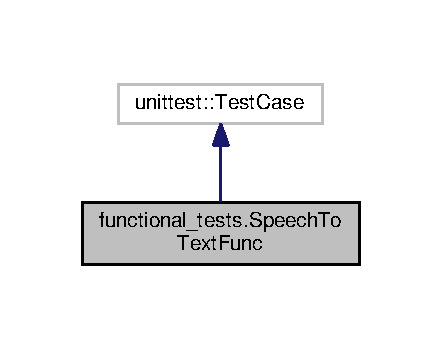
\includegraphics[width=212pt]{classfunctional__tests_1_1SpeechToTextFunc__inherit__graph}
\end{center}
\end{figure}


Collaboration diagram for functional\-\_\-tests.\-Speech\-To\-Text\-Func\-:
\nopagebreak
\begin{figure}[H]
\begin{center}
\leavevmode
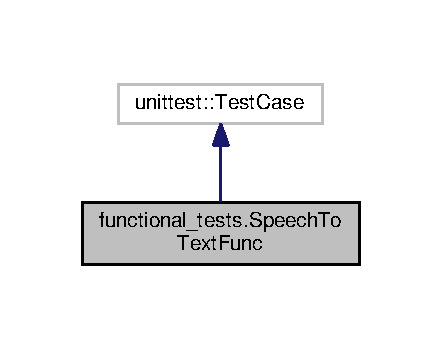
\includegraphics[width=212pt]{classfunctional__tests_1_1SpeechToTextFunc__coll__graph}
\end{center}
\end{figure}
\subsection*{Public Member Functions}
\begin{DoxyCompactItemize}
\item 
def \hyperlink{classfunctional__tests_1_1SpeechToTextFunc_ab33701bb946c7e8c80d8a5b6e7c4abfc}{test\-\_\-image\-File}
\begin{DoxyCompactList}\small\item\em Tests Google A\-S\-R with an image. \end{DoxyCompactList}\item 
def \hyperlink{classfunctional__tests_1_1SpeechToTextFunc_ae5fda4eac95917536723e8134b50a353}{test\-\_\-not\-Existent\-File}
\begin{DoxyCompactList}\small\item\em Tests Google A\-S\-R with a missing file. \end{DoxyCompactList}\item 
def \hyperlink{classfunctional__tests_1_1SpeechToTextFunc_a1038ecffd4b8c2d0ceb9626aedefe2c9}{test\-\_\-wav\-File}
\begin{DoxyCompactList}\small\item\em Tests Google A\-S\-R with a N\-A\-O captured wav file, 1 channel. \end{DoxyCompactList}\item 
def \hyperlink{classfunctional__tests_1_1SpeechToTextFunc_a1c3e6cc84f1bf7ba8efc03f3f602a4f8}{test\-\_\-wav\-File\-\_\-2}
\begin{DoxyCompactList}\small\item\em Tests Google A\-S\-R with a N\-A\-O recorded ogg file. \end{DoxyCompactList}\end{DoxyCompactItemize}


\subsection{Detailed Description}
Inherits the unittest.\-Test\-Case class in order to offer functional tests functionality. 

Definition at line 32 of file functional\-\_\-tests.\-py.



\subsection{Member Function Documentation}
\hypertarget{classfunctional__tests_1_1SpeechToTextFunc_ab33701bb946c7e8c80d8a5b6e7c4abfc}{\index{functional\-\_\-tests\-::\-Speech\-To\-Text\-Func@{functional\-\_\-tests\-::\-Speech\-To\-Text\-Func}!test\-\_\-image\-File@{test\-\_\-image\-File}}
\index{test\-\_\-image\-File@{test\-\_\-image\-File}!functional_tests::SpeechToTextFunc@{functional\-\_\-tests\-::\-Speech\-To\-Text\-Func}}
\subsubsection[{test\-\_\-image\-File}]{\setlength{\rightskip}{0pt plus 5cm}def functional\-\_\-tests.\-Speech\-To\-Text\-Func.\-test\-\_\-image\-File (
\begin{DoxyParamCaption}
\item[{}]{self}
\end{DoxyParamCaption}
)}}\label{classfunctional__tests_1_1SpeechToTextFunc_ab33701bb946c7e8c80d8a5b6e7c4abfc}


Tests Google A\-S\-R with an image. 

Should return nothing 

Definition at line 76 of file functional\-\_\-tests.\-py.

\hypertarget{classfunctional__tests_1_1SpeechToTextFunc_ae5fda4eac95917536723e8134b50a353}{\index{functional\-\_\-tests\-::\-Speech\-To\-Text\-Func@{functional\-\_\-tests\-::\-Speech\-To\-Text\-Func}!test\-\_\-not\-Existent\-File@{test\-\_\-not\-Existent\-File}}
\index{test\-\_\-not\-Existent\-File@{test\-\_\-not\-Existent\-File}!functional_tests::SpeechToTextFunc@{functional\-\_\-tests\-::\-Speech\-To\-Text\-Func}}
\subsubsection[{test\-\_\-not\-Existent\-File}]{\setlength{\rightskip}{0pt plus 5cm}def functional\-\_\-tests.\-Speech\-To\-Text\-Func.\-test\-\_\-not\-Existent\-File (
\begin{DoxyParamCaption}
\item[{}]{self}
\end{DoxyParamCaption}
)}}\label{classfunctional__tests_1_1SpeechToTextFunc_ae5fda4eac95917536723e8134b50a353}


Tests Google A\-S\-R with a missing file. 

Should return nothing 

Definition at line 98 of file functional\-\_\-tests.\-py.

\hypertarget{classfunctional__tests_1_1SpeechToTextFunc_a1038ecffd4b8c2d0ceb9626aedefe2c9}{\index{functional\-\_\-tests\-::\-Speech\-To\-Text\-Func@{functional\-\_\-tests\-::\-Speech\-To\-Text\-Func}!test\-\_\-wav\-File@{test\-\_\-wav\-File}}
\index{test\-\_\-wav\-File@{test\-\_\-wav\-File}!functional_tests::SpeechToTextFunc@{functional\-\_\-tests\-::\-Speech\-To\-Text\-Func}}
\subsubsection[{test\-\_\-wav\-File}]{\setlength{\rightskip}{0pt plus 5cm}def functional\-\_\-tests.\-Speech\-To\-Text\-Func.\-test\-\_\-wav\-File (
\begin{DoxyParamCaption}
\item[{}]{self}
\end{DoxyParamCaption}
)}}\label{classfunctional__tests_1_1SpeechToTextFunc_a1038ecffd4b8c2d0ceb9626aedefe2c9}


Tests Google A\-S\-R with a N\-A\-O captured wav file, 1 channel. 

Should return yes and no 

Definition at line 35 of file functional\-\_\-tests.\-py.

\hypertarget{classfunctional__tests_1_1SpeechToTextFunc_a1c3e6cc84f1bf7ba8efc03f3f602a4f8}{\index{functional\-\_\-tests\-::\-Speech\-To\-Text\-Func@{functional\-\_\-tests\-::\-Speech\-To\-Text\-Func}!test\-\_\-wav\-File\-\_\-2@{test\-\_\-wav\-File\-\_\-2}}
\index{test\-\_\-wav\-File\-\_\-2@{test\-\_\-wav\-File\-\_\-2}!functional_tests::SpeechToTextFunc@{functional\-\_\-tests\-::\-Speech\-To\-Text\-Func}}
\subsubsection[{test\-\_\-wav\-File\-\_\-2}]{\setlength{\rightskip}{0pt plus 5cm}def functional\-\_\-tests.\-Speech\-To\-Text\-Func.\-test\-\_\-wav\-File\-\_\-2 (
\begin{DoxyParamCaption}
\item[{}]{self}
\end{DoxyParamCaption}
)}}\label{classfunctional__tests_1_1SpeechToTextFunc_a1c3e6cc84f1bf7ba8efc03f3f602a4f8}


Tests Google A\-S\-R with a N\-A\-O recorded ogg file. 

Should return \char`\"{}\-Monday\char`\"{} 

Definition at line 56 of file functional\-\_\-tests.\-py.



The documentation for this class was generated from the following file\-:\begin{DoxyCompactItemize}
\item 
/home/travis/rapp\-\_\-temp/rapp-\/platform/rapp\-\_\-speech\-\_\-detection\-\_\-google/tests/speech\-\_\-to\-\_\-text/\hyperlink{functional__tests_8py}{functional\-\_\-tests.\-py}\end{DoxyCompactItemize}

\chapter{File Documentation}
\hypertarget{functional__tests_8py}{\section{/home/travis/rapp\-\_\-temp/rapp-\/platform/rapp\-\_\-speech\-\_\-detection\-\_\-google/tests/speech\-\_\-to\-\_\-text/functional\-\_\-tests.py File Reference}
\label{functional__tests_8py}\index{/home/travis/rapp\-\_\-temp/rapp-\/platform/rapp\-\_\-speech\-\_\-detection\-\_\-google/tests/speech\-\_\-to\-\_\-text/functional\-\_\-tests.\-py@{/home/travis/rapp\-\_\-temp/rapp-\/platform/rapp\-\_\-speech\-\_\-detection\-\_\-google/tests/speech\-\_\-to\-\_\-text/functional\-\_\-tests.\-py}}
}
\subsection*{Classes}
\begin{DoxyCompactItemize}
\item 
class \hyperlink{classfunctional__tests_1_1SpeechToTextFunc}{functional\-\_\-tests.\-Speech\-To\-Text\-Func}
\begin{DoxyCompactList}\small\item\em Inherits the unittest.\-Test\-Case class in order to offer functional tests functionality. \end{DoxyCompactList}\end{DoxyCompactItemize}
\subsection*{Namespaces}
\begin{DoxyCompactItemize}
\item 
\hyperlink{namespacefunctional__tests}{functional\-\_\-tests}
\end{DoxyCompactItemize}
\subsection*{Variables}
\begin{DoxyCompactItemize}
\item 
string \hyperlink{namespacefunctional__tests_a78507f367d6307db1c1633379cbccc35}{functional\-\_\-tests.\-P\-K\-G} = 'rapp\-\_\-speech\-\_\-detection\-\_\-google'
\end{DoxyCompactItemize}

%--- End generated contents ---

% Index
\newpage
\phantomsection
\addcontentsline{toc}{chapter}{Index}
\printindex

\end{document}
